% !TEX program = xelatex
% 2025-2026 学年上海交大附中高一（上）月考化学试卷（10 月份）
% 原文出处：微信公众号「上海初高中化学」2025-09-11
%           https://mp.weixin.qq.com/s/JBr7EYgYrO8DjMwxtt6PAQ
% 排版：XeLaTeX + ctex + chemformula + TikZ
%
% 单文件双输出：
%   试卷版：xelatex 高一化学_交大附中_10月月考.tex
%   答案版：xelatex "\def\isanswer{1}% !TEX program = xelatex
% 2025-2026 学年上海交大附中高一（上）月考化学试卷（10 月份）
% 原文出处：微信公众号「上海初高中化学」2025-09-11
%           https://mp.weixin.qq.com/s/JBr7EYgYrO8DjMwxtt6PAQ
% 排版：XeLaTeX + ctex + chemformula + TikZ
%
% 单文件双输出：
%   试卷版：xelatex 高一化学_交大附中_10月月考.tex
%   答案版：xelatex "\def\isanswer{1}% !TEX program = xelatex
% 2025-2026 学年上海交大附中高一（上）月考化学试卷（10 月份）
% 原文出处：微信公众号「上海初高中化学」2025-09-11
%           https://mp.weixin.qq.com/s/JBr7EYgYrO8DjMwxtt6PAQ
% 排版：XeLaTeX + ctex + chemformula + TikZ
%
% 单文件双输出：
%   试卷版：xelatex 高一化学_交大附中_10月月考.tex
%   答案版：xelatex "\def\isanswer{1}% !TEX program = xelatex
% 2025-2026 学年上海交大附中高一（上）月考化学试卷（10 月份）
% 原文出处：微信公众号「上海初高中化学」2025-09-11
%           https://mp.weixin.qq.com/s/JBr7EYgYrO8DjMwxtt6PAQ
% 排版：XeLaTeX + ctex + chemformula + TikZ
%
% 单文件双输出：
%   试卷版：xelatex 高一化学_交大附中_10月月考.tex
%   答案版：xelatex "\def\isanswer{1}\input{高一化学_交大附中_10月月考.tex}"

\documentclass[11pt,a4paper]{article}
\usepackage{chem}

% ---- 卷名（页眉；答案版自动追加版本标记）----
\newcommand{\paperhead}{2025-2026 学年上海交大附中高一（上）月考化学试卷（10 月份）}
\fancyhead[L]{\small\kaishu \paperhead\vermark}

% ---- 标题 ----
\title{\heiti\bfseries\Large \paperhead}
\author{}
\date{}

\begin{document}
\maketitle
\thispagestyle{fancy}

%==========================================================
\bigsection{一、破解月壤化学之谜（20 分）}

\noindent\textbf{1.（20 分）}2025 年 7 月，中国科学家基于对月壤样品的成分分析，于《自然》期刊上发表了突破性研究，其中所揭示的数据为理解月球背面的岩浆活动、水含量及撞击历史提供了关键证据。

\begin{enumerate}[label=（\arabic*）]
\item \ch{^{3}He} 与 \ch{^{3}H} 发生聚变有可能被开发为能源。\ch{^{3}He} 与 \ch{^{3}H} 具有相同的\blank[2.4em]。
\choice{中子数}{质子数}{质量数}{电子数}

\item 月壤中含有的元素可形成 \ch{^{13}C^{17}O} 分子，有助于揭示行星诞生之谜，下列关于 \ch{^{13}C^{17}O} 和 \ch{^{12}C^{16}O} 的说法正确的是\blank[2.4em]。
\choice{互为同素异形体}{互为同位素}{具有相同的性质}{它们是同种物质}

\item 月壤的构成与地球土壤类似。土壤中含有的 W、X、Y、Z 是 1$\sim$18 号元素中的四种，且原子序数依次增大，最外层电子数之和为 15，其中 W 的最外层电子数是内层电子总数的 3 倍，X、Y、Z 原子序数是连续的。

写出 W 元素的简单离子的电子式\blank[6em]。

\item X 原子核外电子所占据的电子层中，能量最高的是\blank[2.5em]层（填符号）。

\item Y 元素的简单离子结构示意图为\blank[3em]。请写出与它具有相同电子数的四核微粒的化学式\blank[2.5em]（写一个即可）。

\item Z 元素在自然界中有三种稳定的同位素，相关信息如下：

\begin{center}
\begin{tabular}{|c|c|c|c|}
\hline
\rule{0pt}{1.2em}核素符号 & \ch{^{28}Z} & \ch{^{29}Z} & \ch{^{30}Z} \\
\hline
\rule{0pt}{1.2em}相对原子质量 & 27.977 & 28.976 & 29.974 \\
\hline
\rule{0pt}{1.2em}丰度（\%） & $x$ & $y$ & 3.10 \\
\hline
\rule{0pt}{1.2em}Z 元素的平均相对原子质量 & \multicolumn{3}{c|}{28.086} \\
\hline
\end{tabular}
\end{center}

\textcircled{1} 表格中 $x$、$y$ 和 3.10\% 分别代表 Z 中对应核素的丰度，则 $x =$\blank[3.5em] \%，$y =$\blank[3.5em] \%（计算结果保留两位小数）。

\textcircled{2} \ch{^{30}Z} 在自然界的质量分数\blank[2em]3.1\%（填“>”、“<”或“=”），12 g ZO\textsubscript{2} 中 \ch{^{30}Z} 的质量为\blank[3em]（计算结果保留两位小数）。
\end{enumerate}

%==========================================================
\bigsection{二、胶体金检测试剂（20 分）}

\noindent\textbf{2.（20 分）}胶体金（Au）免疫层析法可用于快速检测新型冠状病毒抗体。利用柠檬酸钠溶液还原氯金酸（\ch{HAuCl4}）即可制备得到胶体金。研究发现：柠檬酸钠的用量不同会导致胶体金粒径和颜色的不同。免疫胶体金技术可用于甲型流感病毒的快速免疫筛查，检测原理是胶体金与蛋白质分子的正电荷基团形成牢固的结合体，再通过抗原-抗体结合形成免疫复合物，使得胶体金颗粒聚集，发生颜色变化。

\begin{enumerate}[label=（\arabic*）]
\item 下列说法中错误的是\blank[3em]。
\choice{胶体金颗粒带负电荷}{用半透膜分离胶体金吸附的离子}{胶体金颗粒的团聚过程利用电泳原理}{检测过程胶体金分散质粒子直径不变}

\item 利用超显微镜，可以观察到胶体金颗粒的形态，胶体金分散质粒子的直径大致范围在\blank[4em]m 之间。检验胶体最便利的方法是观察它\blank[4em]。

\item 若将胶体金装入 U 型管中，插入电极后通直流电，发现\blank[2.5em]极（选填“阴”或“阳”）附近颜色加深，产生这一现象的原因是\blank[8em]。

\item 向新冠肺炎自测试剂盒中倒入可乐或柠檬水可能会导致假阳性。推测这一现象的原因：\par\noindent\hspace{2em}\blank[10em]。

\item 与第（4）题现象的原理相同的选项有\blank[3em]。
\choice{长江三角洲的形成}{血液透析}{大雨过后拍到“耶稣光”}{不同品牌的墨水不能混用}

\item 已知等浓度的 \ch{MgSO4} 溶液对胶体金的聚沉效果强于 \ch{NaCl} 溶液，加入等浓度的下列溶液时，聚沉胶体金效果最明显的是\blank[3em]。
\choice{\ch{BaCl2}}{\ch{Al2(SO4)3}}{\ch{KCl}}{\ch{CuSO4}}

\item 请分析该公司根据胶体金免疫层析法研制自测试剂盒的缺陷：\blank[10em]。
\end{enumerate}

%==========================================================
\bigsection{三、物质的量（22 分）}

\noindent\textbf{3.（22 分）}研究含碳物质的转化，对缓解能源危机和实现碳中和具有重要意义。碳和甲烷均可以与水反应用来制取水煤气（\ch{CO}、\ch{H2}），请回答下列问题：

\begin{enumerate}[label=（\arabic*）]
\item 标准状况下，11.2 L \ch{CO} 的摩尔质量为\blank[3.5em]g$\cdot$mol\textsuperscript{$-1$}，分子个数为\blank[4em]。

\item 1 mol \ch{CH4} 中含有的 H 原子个数与\blank[3em]g \ch{H2O} 中含有的 H 原子个数相同。
\choice{36}{18}{72}{9}

\item 下列叙述错误的是\blank[3em]。
\begin{itemize}[leftmargin=2em,itemsep=0.1em]
\item[ \textcircled{1} ] 摩尔是国际单位制中的七个基本物理量之一；
\item[ \textcircled{2} ] 1 mol 任何物质都含有约 $6.02\times 10^{23}$ 个原子；
\item[ \textcircled{3} ] $6.02\times 10^{23}$ 就是阿伏加德罗常数；
\item[ \textcircled{4} ] 碳原子的摩尔质量是 12 g；
\item[ \textcircled{5} ] \ch{CO2} 的摩尔质量等于 1 mol \ch{CO2} 分子的质量；
\item[ \textcircled{6} ] 1 mol \ch{CO2} 中含有 1 mol 碳和 2 mol 氧；
\item[ \textcircled{7} ] 0.012 kg \ch{^{12}C} 中含有 \ch{^{12}C} 的数目为 1 mol。
\end{itemize}
\choice{\textcircled{1}\textcircled{2}\textcircled{3}}{\textcircled{2}\textcircled{3}\textcircled{4}}{\textcircled{2}\textcircled{3}\textcircled{4}\textcircled{6}}{全部}

\item 常温常压下，用等质量的 \ch{CH4}、\ch{CO}、\ch{H2}、\ch{CO2} 四种气体分别吹出四个气球。其中气体为 \ch{CO2} 的是\blank[3em]（填序号）。

\begin{center}
\begin{tikzpicture}
  % 原卷图（截图裁切自 img_2，二值化放大 2 倍）
  \node[anchor=south west,inner sep=0] (img) at (0,0)
    {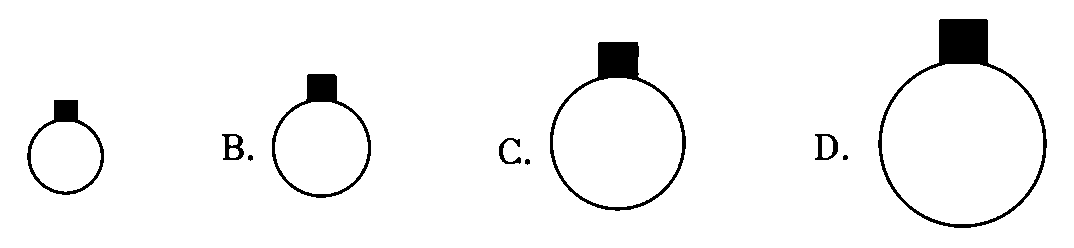
\includegraphics[width=0.80\textwidth]{figures/balloons.png}};
  % 原卷图中未印字母，此处按气球中心位置补注 A/B/C/D
  \foreach \lab/\p in {A/0.0615, B/0.2980, C/0.5754, D/0.8957} {
    \node[below=2pt] at ($(img.south west)!\p!(img.south east)$) {\small\textbf{\lab}};
  }
\end{tikzpicture}
\end{center}

\item 标准状况下，8.96 L \ch{CH4} 和 \ch{CO} 的混合气体总质量为 7.6 g，则混合气体中甲烷的体积为\blank[3em]L，一氧化碳的质量为\blank[3em]g。

\item 同温同压下，17.2 g \ch{N2}、\ch{CO} 和 \ch{CO2} 的混合气体与 4.4 g \ch{CO2} 的体积之比为 5:1。
\begin{enumerate}[label=\textcircled{\arabic*}]
\item 该混合气体的总物质的量为\blank[3em]mol。
\item 该混合气体的平均摩尔质量为\blank[3em]g/mol。
\item 该混合气体中 \ch{CO2} 的质量为\blank[3em]g。
\end{enumerate}

制取水煤气的副产品为 \ch{CO2}，工业中可以利用 \ch{CO2} 合成纯碱。

现有一份纯碱样品，已知其中只含有氯化钠杂质。某化学实验小组为测定样品中碳酸钠的含量进行如下实验：

\noindent 步骤 I：准确称量 21.20 g 纯碱样品，加入适量蒸馏水溶解；\\
步骤 II：向上述溶液中逐滴加入 \ch{CaCl2} 溶液，直至不再产生沉淀为止；\\
步骤 III：将所得混合物过滤、洗涤、干燥，得到 15.00 g 固体。

请计算：

\item 步骤 III 中所得固体的物质的量为\blank[3em]mol。
\choice{0.3}{0.15}{15}{0.135}

\item 样品中 \ch{Na2CO3} 的质量分数为\blank[3em]。
\choice{70.8\%}{78.5\%}{75\%}{25\%}

\item 下列实验方案中，能测定样品中碳酸钠质量分数的是\blank[3em]（双选）。
\begin{itemize}[leftmargin=2em,itemsep=0.1em]
\item[A.] 向步骤 I 所得溶液逐滴加入标准盐酸至恰好不再有气体生成，共消耗 $b$ mol 溶质的稀盐酸。经计算，测得样品中 \ch{Na2CO3} 的质量分数为 $\omega(\ch{Na2CO3}) = \dfrac{53b}{21.20}$。
\item[B.] 向步骤 I 所得溶液中加入足量稀硫酸，将生成的气体用碱石灰吸收，碱石灰增重 $a$ g。经计算，测得样品中 \ch{Na2CO3} 的质量分数为 $\omega(\ch{Na2CO3}) = \dfrac{53a}{22\times 21.20}$。
\item[C.] 向步骤 I 所得溶液中加入硝酸酸化，再加入足量的硝酸银溶液充分反应，过滤、洗涤、干燥，得 $c$ g 固体。经计算，测得样品中 \ch{Na2CO3} 的质量分数为 $\omega(\ch{Na2CO3}) = \left(1 - \dfrac{58.5c}{143.5\times 21.20}\right)$。
\end{itemize}
\end{enumerate}

%==========================================================
\bigsection{四、生理盐水中氯化钠含量的分析（19 分）}

\noindent\textbf{4.（19 分）}生理盐水是渗透压与动物或人体血浆相等的氯化钠溶液，其质量分数为 0.9\%，广泛用于补液，体外细胞培养及医疗操作中。

\begin{enumerate}[label=（\arabic*）]
\item 请计算生理盐水的物质的量浓度为\blank[3.5em]mol/L。（生理盐水密度约等于 1 g/cm\textsuperscript{3}，结果保留三位有效数字）

某同学想要使用如下方法对某市售生理盐水进行浓度分析：
\begin{itemize}[leftmargin=2em,itemsep=0.1em]
\item[ \textcircled{1} ] 配制 0.1000 mol/L 硝酸银溶液 100 mL
\item[ \textcircled{2} ] 取 25.00 mL 生理盐水于锥形瓶中，加入指示剂后使用配制好的硝酸银溶液进行滴定，消耗 36.62 mL。
\end{itemize}
滴定过程中发生的反应：$\mathrm{Ag^{+} + Cl^{-} \longrightarrow AgCl \downarrow}$

\item 计算需称取硝酸银\blank[3.5em]g（结果保留三位有效数字）。

\item 在配制硝酸银溶液实验中，下列不需要使用的仪器是\blank[3em]（填选项），除了玻璃棒和下列选项中出现的仪器外，还需要的玻璃仪器是\blank[4em]。
\choice{250 mL 烧杯}{胶头滴管}{量筒}{电子天平}

\item 配制过程中，玻璃棒使用了两次，其作用分别为\blank[6em]、\blank[6em]。

\item 下列配制硝酸银溶液的主要操作步骤，正确顺序是\blank[3em]。
\begin{itemize}[leftmargin=2em,itemsep=0.1em]
\item[ \textcircled{1} ] 称取一定质量的硝酸银，放入烧杯中，用适量蒸馏水溶解；
\item[ \textcircled{2} ] 加水至液面刻度线下 1$\sim$2 厘米时，改用胶头滴管加蒸馏水至凹液面与刻度线相切；
\item[ \textcircled{3} ] 将溶液转移到容量瓶中；
\item[ \textcircled{4} ] 盖好瓶塞，反复上下颠倒，摇匀；
\item[ \textcircled{5} ] 用少量蒸馏水洗涤烧杯内壁和玻璃棒 2$\sim$3 次，洗涤液转移到容量瓶中。
\end{itemize}
\choice{\textcircled{1}\textcircled{5}\textcircled{3}\textcircled{2}\textcircled{4}}{\textcircled{1}\textcircled{3}\textcircled{2}\textcircled{4}\textcircled{5}}{\textcircled{1}\textcircled{5}\textcircled{3}\textcircled{2}\textcircled{4}}{\textcircled{1}\textcircled{3}\textcircled{5}\textcircled{4}\textcircled{2}}

\item 计算该市售生理盐水的物质的量浓度为\blank[3.5em]mol/L（密度约等于 1 g$\cdot$cm\textsuperscript{$-$3}，结果保留三位有效数字）。

\item 溶液中微粒的总浓度越大，溶液的渗透压越高。人体的血细胞在高渗透压的溶液中会失水皱缩，在低渗透压环境下会吸水膨胀，只有在等渗透压溶液中才能够保持正常。因此诸如生理盐水这样的等渗溶液十分重要。已知 \ch{NaCl} 在溶液中的存在形式为 \ch{Na+} 与 \ch{Cl-}，\ch{Na2SO4} 在溶液中的存在形式为 \ch{Na+} 与 $\mathrm{SO_4^{2-}}$，试判断在 0.12 mol/L 的 \ch{Na2SO4} 溶液中血细胞会怎样：\blank[3em]。
\choicethree{失水皱缩}{吸水膨胀}{保持正常}
\end{enumerate}

%==========================================================
\bigsection{五、紫甘蓝指示剂（18 分）}

\noindent\textbf{5.（19 分）}紫甘蓝与石蕊类似，在酸碱性不同的溶液中均能显示出不同的颜色，因此也被作为酸碱指示剂。以下是紫甘蓝指示剂随溶液 pH 值的变色范围。

\begin{center}
\begin{tabular}{|c|c|c|c|c|c|c|c|}
\hline
\rule{0pt}{1.2em}pH & 1 & 2$\sim$3 & 4$\sim$6 & 7$\sim$9 & 10 & 11 & 12$\sim$14 \\
\hline
\rule{0pt}{1.2em}溶液颜色 & 深红 & 紫红 & 浅紫 & 蓝 & 青 & 绿 & 黄 \\
\hline
\end{tabular}
\end{center}

\begin{enumerate}[label=（\arabic*）]
\item 下列可能使紫甘蓝溶液变为浅紫色的物质有\blank[3em]。
\choice{\ch{NaCl}}{\ch{CH3COOH}}{\ch{Ca(OH)2}}{\ch{K2SO4}}

向一定浓度的碳酸氢钠中滴加几滴紫甘蓝溶液，观察到溶液呈蓝色。向溶液中滴加几滴稀盐酸，观察到有气泡产生，且溶液依然呈蓝色。

\item 碳酸氢钠属于\blank[3em]。
\choice{正盐}{碱式盐}{酸式盐}{复盐}

\item 滴加稀盐酸前的碳酸氢钠溶液呈\blank[3em]。
\choicethree{酸性}{碱性}{中性}

向一定浓度的硫酸氢钠中滴加几滴紫甘蓝溶液，观察到溶液呈紫红色。向溶液中滴加几滴稀硫酸，无明显现象。另取少量硫酸氢钠溶液滴加到碳酸氢钠溶液中，观察到有气泡产生。

\item 下列说法正确的是\blank[3em]。
\choice{硫酸氢钠不是酸式盐}{硫酸氢钠溶液呈碱性}{某些盐类物质可以互相反应}{酸式盐可能显酸性可能显碱性}

\item 写出硫酸氢钠与碳酸氢钠溶液反应的化学方程式\blank[10em]。

向盛有 0.2 mol 硫酸氢钠溶液的烧杯中加入碳酸钡固体，当加入 $a$ g 碳酸钡固体后，产生了 0.05 mol 气体（假设 \ch{CO2} 全部逸出）。

\item $a =$\blank[4em]。

\item 此时溶液中的溶质为\blank[6em]。

\item 继续加入碳酸钡固体，当烧杯中恰好有 23.3 g 固体时，向烧杯中滴加几滴紫甘蓝溶液，溶液呈\blank[2em]色。
\end{enumerate}

%==========================================================
% 以下「参考答案」整节仅在答案版输出（试卷版由 \ifanswer 整段吞掉）
\ifanswer
\newpage
\bigsection{参考答案}

\begin{enumerate}[label=\textbf{\arabic*.},leftmargin=2.5em]
\item
\begin{enumerate}[label=（\arabic*）]
\item A（原卷参考答案写作“A”；\ch{^{3}He} 与 \ch{^{3}H} 的中子数为 1 与 2、质子数为 2 与 1，均不相同，相同的是质量数 3，按题意应为 C）；
\item D；
\item $\left[:\ddot{\mathrm{O}}:\right]^{2-}$（O\textsuperscript{2-} 的电子式）；
\item M；
\item Al\textsuperscript{3+} 的结构示意图为
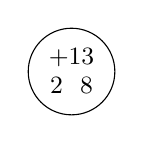
\begin{tikzpicture}[baseline=-0.5ex]
\draw (0,0) circle (0.55);
\node at (0,0.18) {\small $+13$};
\node at (0,-0.18) {\small $2\ \ 8$};
\end{tikzpicture}；相同电子数（10 e\textsuperscript{$-$}) 的四核微粒：\ch{NH3} 或 \ch{CH4}（答案给的是 \ch{PH3}，疑为 \ch{NH3} 之误）；
\item \textcircled{1} $x = 92.18$\%，$y = 4.72$\%（原卷参考答案写作“83.18；13.72”，按算式复核应为上述数值）；\textcircled{2} $>$；0.19 g。
\end{enumerate}

\item
\begin{enumerate}[label=（\arabic*）]
\item CD；
\item $1\times 10^{-9} \sim 1\times 10^{-7}$ m；丁达尔效应；
\item 阳；胶体粒子带负电荷，通电发生电泳向阳极移动；
\item 胶体遇其他电解质溶液发生了聚沉；
\item AD；
\item B；
\item 不稳定，易受外界环境影响。
\end{enumerate}

\item
\begin{enumerate}[label=（\arabic*）]
\item 28 g$\cdot$mol\textsuperscript{$-$1}；$0.5N_A$；
\item A；
\item D；
\item A（原卷参考答案写作“B”，按物理推算应为 A：等质量下 $V\propto 1/\rho$，$\rho(\mathrm{CO_2})=1.96$ 最大，故 \ch{CO2} 气球最小）；
\item 6.72 L；2.8 g；
\item \textcircled{1} 0.5 mol；\textcircled{2} 34.4 g/mol；\textcircled{3} 8.8 g；
\item B；
\item C；
\item AC。
\end{enumerate}

\item
\begin{enumerate}[label=（\arabic*）]
\item 0.154；
\item 1.70；
\item C；100 mL 容量瓶；
\item 搅拌，加速溶解；引流，防止溶液漏出；
\item C；
\item 0.146；
\item A。
\end{enumerate}

\item
\begin{enumerate}[label=（\arabic*）]
\item B；
\item C；
\item B；
\item CD；
\item $\mathrm{NaHCO_3 + NaHSO_4 \longrightarrow Na_2SO_4 + H_2O + CO_2 \uparrow}$；
\item 9.85；
\item 硫酸氢钠和硫酸钠；
\item 蓝。
\end{enumerate}
\end{enumerate}
\fi

\end{document}
"

\documentclass[11pt,a4paper]{article}
\usepackage{chem}

% ---- 卷名（页眉；答案版自动追加版本标记）----
\newcommand{\paperhead}{2025-2026 学年上海交大附中高一（上）月考化学试卷（10 月份）}
\fancyhead[L]{\small\kaishu \paperhead\vermark}

% ---- 标题 ----
\title{\heiti\bfseries\Large \paperhead}
\author{}
\date{}

\begin{document}
\maketitle
\thispagestyle{fancy}

%==========================================================
\bigsection{一、破解月壤化学之谜（20 分）}

\noindent\textbf{1.（20 分）}2025 年 7 月，中国科学家基于对月壤样品的成分分析，于《自然》期刊上发表了突破性研究，其中所揭示的数据为理解月球背面的岩浆活动、水含量及撞击历史提供了关键证据。

\begin{enumerate}[label=（\arabic*）]
\item \ch{^{3}He} 与 \ch{^{3}H} 发生聚变有可能被开发为能源。\ch{^{3}He} 与 \ch{^{3}H} 具有相同的\blank[2.4em]。
\choice{中子数}{质子数}{质量数}{电子数}

\item 月壤中含有的元素可形成 \ch{^{13}C^{17}O} 分子，有助于揭示行星诞生之谜，下列关于 \ch{^{13}C^{17}O} 和 \ch{^{12}C^{16}O} 的说法正确的是\blank[2.4em]。
\choice{互为同素异形体}{互为同位素}{具有相同的性质}{它们是同种物质}

\item 月壤的构成与地球土壤类似。土壤中含有的 W、X、Y、Z 是 1$\sim$18 号元素中的四种，且原子序数依次增大，最外层电子数之和为 15，其中 W 的最外层电子数是内层电子总数的 3 倍，X、Y、Z 原子序数是连续的。

写出 W 元素的简单离子的电子式\blank[6em]。

\item X 原子核外电子所占据的电子层中，能量最高的是\blank[2.5em]层（填符号）。

\item Y 元素的简单离子结构示意图为\blank[3em]。请写出与它具有相同电子数的四核微粒的化学式\blank[2.5em]（写一个即可）。

\item Z 元素在自然界中有三种稳定的同位素，相关信息如下：

\begin{center}
\begin{tabular}{|c|c|c|c|}
\hline
\rule{0pt}{1.2em}核素符号 & \ch{^{28}Z} & \ch{^{29}Z} & \ch{^{30}Z} \\
\hline
\rule{0pt}{1.2em}相对原子质量 & 27.977 & 28.976 & 29.974 \\
\hline
\rule{0pt}{1.2em}丰度（\%） & $x$ & $y$ & 3.10 \\
\hline
\rule{0pt}{1.2em}Z 元素的平均相对原子质量 & \multicolumn{3}{c|}{28.086} \\
\hline
\end{tabular}
\end{center}

\textcircled{1} 表格中 $x$、$y$ 和 3.10\% 分别代表 Z 中对应核素的丰度，则 $x =$\blank[3.5em] \%，$y =$\blank[3.5em] \%（计算结果保留两位小数）。

\textcircled{2} \ch{^{30}Z} 在自然界的质量分数\blank[2em]3.1\%（填“>”、“<”或“=”），12 g ZO\textsubscript{2} 中 \ch{^{30}Z} 的质量为\blank[3em]（计算结果保留两位小数）。
\end{enumerate}

%==========================================================
\bigsection{二、胶体金检测试剂（20 分）}

\noindent\textbf{2.（20 分）}胶体金（Au）免疫层析法可用于快速检测新型冠状病毒抗体。利用柠檬酸钠溶液还原氯金酸（\ch{HAuCl4}）即可制备得到胶体金。研究发现：柠檬酸钠的用量不同会导致胶体金粒径和颜色的不同。免疫胶体金技术可用于甲型流感病毒的快速免疫筛查，检测原理是胶体金与蛋白质分子的正电荷基团形成牢固的结合体，再通过抗原-抗体结合形成免疫复合物，使得胶体金颗粒聚集，发生颜色变化。

\begin{enumerate}[label=（\arabic*）]
\item 下列说法中错误的是\blank[3em]。
\choice{胶体金颗粒带负电荷}{用半透膜分离胶体金吸附的离子}{胶体金颗粒的团聚过程利用电泳原理}{检测过程胶体金分散质粒子直径不变}

\item 利用超显微镜，可以观察到胶体金颗粒的形态，胶体金分散质粒子的直径大致范围在\blank[4em]m 之间。检验胶体最便利的方法是观察它\blank[4em]。

\item 若将胶体金装入 U 型管中，插入电极后通直流电，发现\blank[2.5em]极（选填“阴”或“阳”）附近颜色加深，产生这一现象的原因是\blank[8em]。

\item 向新冠肺炎自测试剂盒中倒入可乐或柠檬水可能会导致假阳性。推测这一现象的原因：\par\noindent\hspace{2em}\blank[10em]。

\item 与第（4）题现象的原理相同的选项有\blank[3em]。
\choice{长江三角洲的形成}{血液透析}{大雨过后拍到“耶稣光”}{不同品牌的墨水不能混用}

\item 已知等浓度的 \ch{MgSO4} 溶液对胶体金的聚沉效果强于 \ch{NaCl} 溶液，加入等浓度的下列溶液时，聚沉胶体金效果最明显的是\blank[3em]。
\choice{\ch{BaCl2}}{\ch{Al2(SO4)3}}{\ch{KCl}}{\ch{CuSO4}}

\item 请分析该公司根据胶体金免疫层析法研制自测试剂盒的缺陷：\blank[10em]。
\end{enumerate}

%==========================================================
\bigsection{三、物质的量（22 分）}

\noindent\textbf{3.（22 分）}研究含碳物质的转化，对缓解能源危机和实现碳中和具有重要意义。碳和甲烷均可以与水反应用来制取水煤气（\ch{CO}、\ch{H2}），请回答下列问题：

\begin{enumerate}[label=（\arabic*）]
\item 标准状况下，11.2 L \ch{CO} 的摩尔质量为\blank[3.5em]g$\cdot$mol\textsuperscript{$-1$}，分子个数为\blank[4em]。

\item 1 mol \ch{CH4} 中含有的 H 原子个数与\blank[3em]g \ch{H2O} 中含有的 H 原子个数相同。
\choice{36}{18}{72}{9}

\item 下列叙述错误的是\blank[3em]。
\begin{itemize}[leftmargin=2em,itemsep=0.1em]
\item[ \textcircled{1} ] 摩尔是国际单位制中的七个基本物理量之一；
\item[ \textcircled{2} ] 1 mol 任何物质都含有约 $6.02\times 10^{23}$ 个原子；
\item[ \textcircled{3} ] $6.02\times 10^{23}$ 就是阿伏加德罗常数；
\item[ \textcircled{4} ] 碳原子的摩尔质量是 12 g；
\item[ \textcircled{5} ] \ch{CO2} 的摩尔质量等于 1 mol \ch{CO2} 分子的质量；
\item[ \textcircled{6} ] 1 mol \ch{CO2} 中含有 1 mol 碳和 2 mol 氧；
\item[ \textcircled{7} ] 0.012 kg \ch{^{12}C} 中含有 \ch{^{12}C} 的数目为 1 mol。
\end{itemize}
\choice{\textcircled{1}\textcircled{2}\textcircled{3}}{\textcircled{2}\textcircled{3}\textcircled{4}}{\textcircled{2}\textcircled{3}\textcircled{4}\textcircled{6}}{全部}

\item 常温常压下，用等质量的 \ch{CH4}、\ch{CO}、\ch{H2}、\ch{CO2} 四种气体分别吹出四个气球。其中气体为 \ch{CO2} 的是\blank[3em]（填序号）。

\begin{center}
\begin{tikzpicture}
  % 原卷图（截图裁切自 img_2，二值化放大 2 倍）
  \node[anchor=south west,inner sep=0] (img) at (0,0)
    {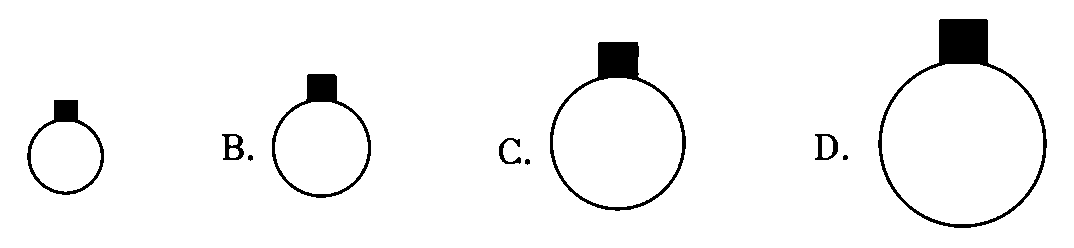
\includegraphics[width=0.80\textwidth]{figures/balloons.png}};
  % 原卷图中未印字母，此处按气球中心位置补注 A/B/C/D
  \foreach \lab/\p in {A/0.0615, B/0.2980, C/0.5754, D/0.8957} {
    \node[below=2pt] at ($(img.south west)!\p!(img.south east)$) {\small\textbf{\lab}};
  }
\end{tikzpicture}
\end{center}

\item 标准状况下，8.96 L \ch{CH4} 和 \ch{CO} 的混合气体总质量为 7.6 g，则混合气体中甲烷的体积为\blank[3em]L，一氧化碳的质量为\blank[3em]g。

\item 同温同压下，17.2 g \ch{N2}、\ch{CO} 和 \ch{CO2} 的混合气体与 4.4 g \ch{CO2} 的体积之比为 5:1。
\begin{enumerate}[label=\textcircled{\arabic*}]
\item 该混合气体的总物质的量为\blank[3em]mol。
\item 该混合气体的平均摩尔质量为\blank[3em]g/mol。
\item 该混合气体中 \ch{CO2} 的质量为\blank[3em]g。
\end{enumerate}

制取水煤气的副产品为 \ch{CO2}，工业中可以利用 \ch{CO2} 合成纯碱。

现有一份纯碱样品，已知其中只含有氯化钠杂质。某化学实验小组为测定样品中碳酸钠的含量进行如下实验：

\noindent 步骤 I：准确称量 21.20 g 纯碱样品，加入适量蒸馏水溶解；\\
步骤 II：向上述溶液中逐滴加入 \ch{CaCl2} 溶液，直至不再产生沉淀为止；\\
步骤 III：将所得混合物过滤、洗涤、干燥，得到 15.00 g 固体。

请计算：

\item 步骤 III 中所得固体的物质的量为\blank[3em]mol。
\choice{0.3}{0.15}{15}{0.135}

\item 样品中 \ch{Na2CO3} 的质量分数为\blank[3em]。
\choice{70.8\%}{78.5\%}{75\%}{25\%}

\item 下列实验方案中，能测定样品中碳酸钠质量分数的是\blank[3em]（双选）。
\begin{itemize}[leftmargin=2em,itemsep=0.1em]
\item[A.] 向步骤 I 所得溶液逐滴加入标准盐酸至恰好不再有气体生成，共消耗 $b$ mol 溶质的稀盐酸。经计算，测得样品中 \ch{Na2CO3} 的质量分数为 $\omega(\ch{Na2CO3}) = \dfrac{53b}{21.20}$。
\item[B.] 向步骤 I 所得溶液中加入足量稀硫酸，将生成的气体用碱石灰吸收，碱石灰增重 $a$ g。经计算，测得样品中 \ch{Na2CO3} 的质量分数为 $\omega(\ch{Na2CO3}) = \dfrac{53a}{22\times 21.20}$。
\item[C.] 向步骤 I 所得溶液中加入硝酸酸化，再加入足量的硝酸银溶液充分反应，过滤、洗涤、干燥，得 $c$ g 固体。经计算，测得样品中 \ch{Na2CO3} 的质量分数为 $\omega(\ch{Na2CO3}) = \left(1 - \dfrac{58.5c}{143.5\times 21.20}\right)$。
\end{itemize}
\end{enumerate}

%==========================================================
\bigsection{四、生理盐水中氯化钠含量的分析（19 分）}

\noindent\textbf{4.（19 分）}生理盐水是渗透压与动物或人体血浆相等的氯化钠溶液，其质量分数为 0.9\%，广泛用于补液，体外细胞培养及医疗操作中。

\begin{enumerate}[label=（\arabic*）]
\item 请计算生理盐水的物质的量浓度为\blank[3.5em]mol/L。（生理盐水密度约等于 1 g/cm\textsuperscript{3}，结果保留三位有效数字）

某同学想要使用如下方法对某市售生理盐水进行浓度分析：
\begin{itemize}[leftmargin=2em,itemsep=0.1em]
\item[ \textcircled{1} ] 配制 0.1000 mol/L 硝酸银溶液 100 mL
\item[ \textcircled{2} ] 取 25.00 mL 生理盐水于锥形瓶中，加入指示剂后使用配制好的硝酸银溶液进行滴定，消耗 36.62 mL。
\end{itemize}
滴定过程中发生的反应：$\mathrm{Ag^{+} + Cl^{-} \longrightarrow AgCl \downarrow}$

\item 计算需称取硝酸银\blank[3.5em]g（结果保留三位有效数字）。

\item 在配制硝酸银溶液实验中，下列不需要使用的仪器是\blank[3em]（填选项），除了玻璃棒和下列选项中出现的仪器外，还需要的玻璃仪器是\blank[4em]。
\choice{250 mL 烧杯}{胶头滴管}{量筒}{电子天平}

\item 配制过程中，玻璃棒使用了两次，其作用分别为\blank[6em]、\blank[6em]。

\item 下列配制硝酸银溶液的主要操作步骤，正确顺序是\blank[3em]。
\begin{itemize}[leftmargin=2em,itemsep=0.1em]
\item[ \textcircled{1} ] 称取一定质量的硝酸银，放入烧杯中，用适量蒸馏水溶解；
\item[ \textcircled{2} ] 加水至液面刻度线下 1$\sim$2 厘米时，改用胶头滴管加蒸馏水至凹液面与刻度线相切；
\item[ \textcircled{3} ] 将溶液转移到容量瓶中；
\item[ \textcircled{4} ] 盖好瓶塞，反复上下颠倒，摇匀；
\item[ \textcircled{5} ] 用少量蒸馏水洗涤烧杯内壁和玻璃棒 2$\sim$3 次，洗涤液转移到容量瓶中。
\end{itemize}
\choice{\textcircled{1}\textcircled{5}\textcircled{3}\textcircled{2}\textcircled{4}}{\textcircled{1}\textcircled{3}\textcircled{2}\textcircled{4}\textcircled{5}}{\textcircled{1}\textcircled{5}\textcircled{3}\textcircled{2}\textcircled{4}}{\textcircled{1}\textcircled{3}\textcircled{5}\textcircled{4}\textcircled{2}}

\item 计算该市售生理盐水的物质的量浓度为\blank[3.5em]mol/L（密度约等于 1 g$\cdot$cm\textsuperscript{$-$3}，结果保留三位有效数字）。

\item 溶液中微粒的总浓度越大，溶液的渗透压越高。人体的血细胞在高渗透压的溶液中会失水皱缩，在低渗透压环境下会吸水膨胀，只有在等渗透压溶液中才能够保持正常。因此诸如生理盐水这样的等渗溶液十分重要。已知 \ch{NaCl} 在溶液中的存在形式为 \ch{Na+} 与 \ch{Cl-}，\ch{Na2SO4} 在溶液中的存在形式为 \ch{Na+} 与 $\mathrm{SO_4^{2-}}$，试判断在 0.12 mol/L 的 \ch{Na2SO4} 溶液中血细胞会怎样：\blank[3em]。
\choicethree{失水皱缩}{吸水膨胀}{保持正常}
\end{enumerate}

%==========================================================
\bigsection{五、紫甘蓝指示剂（18 分）}

\noindent\textbf{5.（19 分）}紫甘蓝与石蕊类似，在酸碱性不同的溶液中均能显示出不同的颜色，因此也被作为酸碱指示剂。以下是紫甘蓝指示剂随溶液 pH 值的变色范围。

\begin{center}
\begin{tabular}{|c|c|c|c|c|c|c|c|}
\hline
\rule{0pt}{1.2em}pH & 1 & 2$\sim$3 & 4$\sim$6 & 7$\sim$9 & 10 & 11 & 12$\sim$14 \\
\hline
\rule{0pt}{1.2em}溶液颜色 & 深红 & 紫红 & 浅紫 & 蓝 & 青 & 绿 & 黄 \\
\hline
\end{tabular}
\end{center}

\begin{enumerate}[label=（\arabic*）]
\item 下列可能使紫甘蓝溶液变为浅紫色的物质有\blank[3em]。
\choice{\ch{NaCl}}{\ch{CH3COOH}}{\ch{Ca(OH)2}}{\ch{K2SO4}}

向一定浓度的碳酸氢钠中滴加几滴紫甘蓝溶液，观察到溶液呈蓝色。向溶液中滴加几滴稀盐酸，观察到有气泡产生，且溶液依然呈蓝色。

\item 碳酸氢钠属于\blank[3em]。
\choice{正盐}{碱式盐}{酸式盐}{复盐}

\item 滴加稀盐酸前的碳酸氢钠溶液呈\blank[3em]。
\choicethree{酸性}{碱性}{中性}

向一定浓度的硫酸氢钠中滴加几滴紫甘蓝溶液，观察到溶液呈紫红色。向溶液中滴加几滴稀硫酸，无明显现象。另取少量硫酸氢钠溶液滴加到碳酸氢钠溶液中，观察到有气泡产生。

\item 下列说法正确的是\blank[3em]。
\choice{硫酸氢钠不是酸式盐}{硫酸氢钠溶液呈碱性}{某些盐类物质可以互相反应}{酸式盐可能显酸性可能显碱性}

\item 写出硫酸氢钠与碳酸氢钠溶液反应的化学方程式\blank[10em]。

向盛有 0.2 mol 硫酸氢钠溶液的烧杯中加入碳酸钡固体，当加入 $a$ g 碳酸钡固体后，产生了 0.05 mol 气体（假设 \ch{CO2} 全部逸出）。

\item $a =$\blank[4em]。

\item 此时溶液中的溶质为\blank[6em]。

\item 继续加入碳酸钡固体，当烧杯中恰好有 23.3 g 固体时，向烧杯中滴加几滴紫甘蓝溶液，溶液呈\blank[2em]色。
\end{enumerate}

%==========================================================
% 以下「参考答案」整节仅在答案版输出（试卷版由 \ifanswer 整段吞掉）
\ifanswer
\newpage
\bigsection{参考答案}

\begin{enumerate}[label=\textbf{\arabic*.},leftmargin=2.5em]
\item
\begin{enumerate}[label=（\arabic*）]
\item A（原卷参考答案写作“A”；\ch{^{3}He} 与 \ch{^{3}H} 的中子数为 1 与 2、质子数为 2 与 1，均不相同，相同的是质量数 3，按题意应为 C）；
\item D；
\item $\left[:\ddot{\mathrm{O}}:\right]^{2-}$（O\textsuperscript{2-} 的电子式）；
\item M；
\item Al\textsuperscript{3+} 的结构示意图为
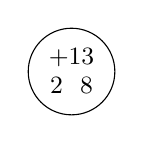
\begin{tikzpicture}[baseline=-0.5ex]
\draw (0,0) circle (0.55);
\node at (0,0.18) {\small $+13$};
\node at (0,-0.18) {\small $2\ \ 8$};
\end{tikzpicture}；相同电子数（10 e\textsuperscript{$-$}) 的四核微粒：\ch{NH3} 或 \ch{CH4}（答案给的是 \ch{PH3}，疑为 \ch{NH3} 之误）；
\item \textcircled{1} $x = 92.18$\%，$y = 4.72$\%（原卷参考答案写作“83.18；13.72”，按算式复核应为上述数值）；\textcircled{2} $>$；0.19 g。
\end{enumerate}

\item
\begin{enumerate}[label=（\arabic*）]
\item CD；
\item $1\times 10^{-9} \sim 1\times 10^{-7}$ m；丁达尔效应；
\item 阳；胶体粒子带负电荷，通电发生电泳向阳极移动；
\item 胶体遇其他电解质溶液发生了聚沉；
\item AD；
\item B；
\item 不稳定，易受外界环境影响。
\end{enumerate}

\item
\begin{enumerate}[label=（\arabic*）]
\item 28 g$\cdot$mol\textsuperscript{$-$1}；$0.5N_A$；
\item A；
\item D；
\item A（原卷参考答案写作“B”，按物理推算应为 A：等质量下 $V\propto 1/\rho$，$\rho(\mathrm{CO_2})=1.96$ 最大，故 \ch{CO2} 气球最小）；
\item 6.72 L；2.8 g；
\item \textcircled{1} 0.5 mol；\textcircled{2} 34.4 g/mol；\textcircled{3} 8.8 g；
\item B；
\item C；
\item AC。
\end{enumerate}

\item
\begin{enumerate}[label=（\arabic*）]
\item 0.154；
\item 1.70；
\item C；100 mL 容量瓶；
\item 搅拌，加速溶解；引流，防止溶液漏出；
\item C；
\item 0.146；
\item A。
\end{enumerate}

\item
\begin{enumerate}[label=（\arabic*）]
\item B；
\item C；
\item B；
\item CD；
\item $\mathrm{NaHCO_3 + NaHSO_4 \longrightarrow Na_2SO_4 + H_2O + CO_2 \uparrow}$；
\item 9.85；
\item 硫酸氢钠和硫酸钠；
\item 蓝。
\end{enumerate}
\end{enumerate}
\fi

\end{document}
"

\documentclass[11pt,a4paper]{article}
\usepackage{chem}

% ---- 卷名（页眉；答案版自动追加版本标记）----
\newcommand{\paperhead}{2025-2026 学年上海交大附中高一（上）月考化学试卷（10 月份）}
\fancyhead[L]{\small\kaishu \paperhead\vermark}

% ---- 标题 ----
\title{\heiti\bfseries\Large \paperhead}
\author{}
\date{}

\begin{document}
\maketitle
\thispagestyle{fancy}

%==========================================================
\bigsection{一、破解月壤化学之谜（20 分）}

\noindent\textbf{1.（20 分）}2025 年 7 月，中国科学家基于对月壤样品的成分分析，于《自然》期刊上发表了突破性研究，其中所揭示的数据为理解月球背面的岩浆活动、水含量及撞击历史提供了关键证据。

\begin{enumerate}[label=（\arabic*）]
\item \ch{^{3}He} 与 \ch{^{3}H} 发生聚变有可能被开发为能源。\ch{^{3}He} 与 \ch{^{3}H} 具有相同的\blank[2.4em]。
\choice{中子数}{质子数}{质量数}{电子数}

\item 月壤中含有的元素可形成 \ch{^{13}C^{17}O} 分子，有助于揭示行星诞生之谜，下列关于 \ch{^{13}C^{17}O} 和 \ch{^{12}C^{16}O} 的说法正确的是\blank[2.4em]。
\choice{互为同素异形体}{互为同位素}{具有相同的性质}{它们是同种物质}

\item 月壤的构成与地球土壤类似。土壤中含有的 W、X、Y、Z 是 1$\sim$18 号元素中的四种，且原子序数依次增大，最外层电子数之和为 15，其中 W 的最外层电子数是内层电子总数的 3 倍，X、Y、Z 原子序数是连续的。

写出 W 元素的简单离子的电子式\blank[6em]。

\item X 原子核外电子所占据的电子层中，能量最高的是\blank[2.5em]层（填符号）。

\item Y 元素的简单离子结构示意图为\blank[3em]。请写出与它具有相同电子数的四核微粒的化学式\blank[2.5em]（写一个即可）。

\item Z 元素在自然界中有三种稳定的同位素，相关信息如下：

\begin{center}
\begin{tabular}{|c|c|c|c|}
\hline
\rule{0pt}{1.2em}核素符号 & \ch{^{28}Z} & \ch{^{29}Z} & \ch{^{30}Z} \\
\hline
\rule{0pt}{1.2em}相对原子质量 & 27.977 & 28.976 & 29.974 \\
\hline
\rule{0pt}{1.2em}丰度（\%） & $x$ & $y$ & 3.10 \\
\hline
\rule{0pt}{1.2em}Z 元素的平均相对原子质量 & \multicolumn{3}{c|}{28.086} \\
\hline
\end{tabular}
\end{center}

\textcircled{1} 表格中 $x$、$y$ 和 3.10\% 分别代表 Z 中对应核素的丰度，则 $x =$\blank[3.5em] \%，$y =$\blank[3.5em] \%（计算结果保留两位小数）。

\textcircled{2} \ch{^{30}Z} 在自然界的质量分数\blank[2em]3.1\%（填“>”、“<”或“=”），12 g ZO\textsubscript{2} 中 \ch{^{30}Z} 的质量为\blank[3em]（计算结果保留两位小数）。
\end{enumerate}

%==========================================================
\bigsection{二、胶体金检测试剂（20 分）}

\noindent\textbf{2.（20 分）}胶体金（Au）免疫层析法可用于快速检测新型冠状病毒抗体。利用柠檬酸钠溶液还原氯金酸（\ch{HAuCl4}）即可制备得到胶体金。研究发现：柠檬酸钠的用量不同会导致胶体金粒径和颜色的不同。免疫胶体金技术可用于甲型流感病毒的快速免疫筛查，检测原理是胶体金与蛋白质分子的正电荷基团形成牢固的结合体，再通过抗原-抗体结合形成免疫复合物，使得胶体金颗粒聚集，发生颜色变化。

\begin{enumerate}[label=（\arabic*）]
\item 下列说法中错误的是\blank[3em]。
\choice{胶体金颗粒带负电荷}{用半透膜分离胶体金吸附的离子}{胶体金颗粒的团聚过程利用电泳原理}{检测过程胶体金分散质粒子直径不变}

\item 利用超显微镜，可以观察到胶体金颗粒的形态，胶体金分散质粒子的直径大致范围在\blank[4em]m 之间。检验胶体最便利的方法是观察它\blank[4em]。

\item 若将胶体金装入 U 型管中，插入电极后通直流电，发现\blank[2.5em]极（选填“阴”或“阳”）附近颜色加深，产生这一现象的原因是\blank[8em]。

\item 向新冠肺炎自测试剂盒中倒入可乐或柠檬水可能会导致假阳性。推测这一现象的原因：\par\noindent\hspace{2em}\blank[10em]。

\item 与第（4）题现象的原理相同的选项有\blank[3em]。
\choice{长江三角洲的形成}{血液透析}{大雨过后拍到“耶稣光”}{不同品牌的墨水不能混用}

\item 已知等浓度的 \ch{MgSO4} 溶液对胶体金的聚沉效果强于 \ch{NaCl} 溶液，加入等浓度的下列溶液时，聚沉胶体金效果最明显的是\blank[3em]。
\choice{\ch{BaCl2}}{\ch{Al2(SO4)3}}{\ch{KCl}}{\ch{CuSO4}}

\item 请分析该公司根据胶体金免疫层析法研制自测试剂盒的缺陷：\blank[10em]。
\end{enumerate}

%==========================================================
\bigsection{三、物质的量（22 分）}

\noindent\textbf{3.（22 分）}研究含碳物质的转化，对缓解能源危机和实现碳中和具有重要意义。碳和甲烷均可以与水反应用来制取水煤气（\ch{CO}、\ch{H2}），请回答下列问题：

\begin{enumerate}[label=（\arabic*）]
\item 标准状况下，11.2 L \ch{CO} 的摩尔质量为\blank[3.5em]g$\cdot$mol\textsuperscript{$-1$}，分子个数为\blank[4em]。

\item 1 mol \ch{CH4} 中含有的 H 原子个数与\blank[3em]g \ch{H2O} 中含有的 H 原子个数相同。
\choice{36}{18}{72}{9}

\item 下列叙述错误的是\blank[3em]。
\begin{itemize}[leftmargin=2em,itemsep=0.1em]
\item[ \textcircled{1} ] 摩尔是国际单位制中的七个基本物理量之一；
\item[ \textcircled{2} ] 1 mol 任何物质都含有约 $6.02\times 10^{23}$ 个原子；
\item[ \textcircled{3} ] $6.02\times 10^{23}$ 就是阿伏加德罗常数；
\item[ \textcircled{4} ] 碳原子的摩尔质量是 12 g；
\item[ \textcircled{5} ] \ch{CO2} 的摩尔质量等于 1 mol \ch{CO2} 分子的质量；
\item[ \textcircled{6} ] 1 mol \ch{CO2} 中含有 1 mol 碳和 2 mol 氧；
\item[ \textcircled{7} ] 0.012 kg \ch{^{12}C} 中含有 \ch{^{12}C} 的数目为 1 mol。
\end{itemize}
\choice{\textcircled{1}\textcircled{2}\textcircled{3}}{\textcircled{2}\textcircled{3}\textcircled{4}}{\textcircled{2}\textcircled{3}\textcircled{4}\textcircled{6}}{全部}

\item 常温常压下，用等质量的 \ch{CH4}、\ch{CO}、\ch{H2}、\ch{CO2} 四种气体分别吹出四个气球。其中气体为 \ch{CO2} 的是\blank[3em]（填序号）。

\begin{center}
\begin{tikzpicture}
  % 原卷图（截图裁切自 img_2，二值化放大 2 倍）
  \node[anchor=south west,inner sep=0] (img) at (0,0)
    {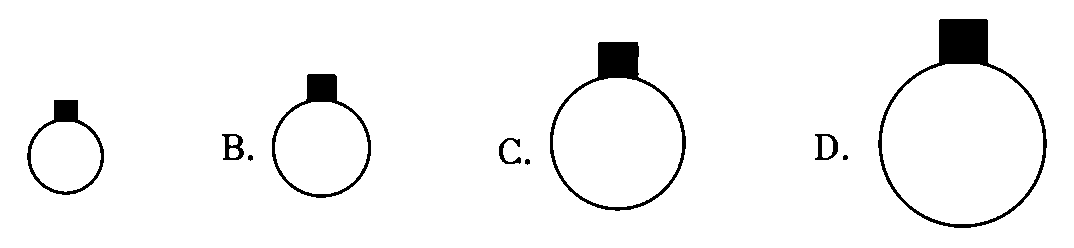
\includegraphics[width=0.80\textwidth]{figures/balloons.png}};
  % 原卷图中未印字母，此处按气球中心位置补注 A/B/C/D
  \foreach \lab/\p in {A/0.0615, B/0.2980, C/0.5754, D/0.8957} {
    \node[below=2pt] at ($(img.south west)!\p!(img.south east)$) {\small\textbf{\lab}};
  }
\end{tikzpicture}
\end{center}

\item 标准状况下，8.96 L \ch{CH4} 和 \ch{CO} 的混合气体总质量为 7.6 g，则混合气体中甲烷的体积为\blank[3em]L，一氧化碳的质量为\blank[3em]g。

\item 同温同压下，17.2 g \ch{N2}、\ch{CO} 和 \ch{CO2} 的混合气体与 4.4 g \ch{CO2} 的体积之比为 5:1。
\begin{enumerate}[label=\textcircled{\arabic*}]
\item 该混合气体的总物质的量为\blank[3em]mol。
\item 该混合气体的平均摩尔质量为\blank[3em]g/mol。
\item 该混合气体中 \ch{CO2} 的质量为\blank[3em]g。
\end{enumerate}

制取水煤气的副产品为 \ch{CO2}，工业中可以利用 \ch{CO2} 合成纯碱。

现有一份纯碱样品，已知其中只含有氯化钠杂质。某化学实验小组为测定样品中碳酸钠的含量进行如下实验：

\noindent 步骤 I：准确称量 21.20 g 纯碱样品，加入适量蒸馏水溶解；\\
步骤 II：向上述溶液中逐滴加入 \ch{CaCl2} 溶液，直至不再产生沉淀为止；\\
步骤 III：将所得混合物过滤、洗涤、干燥，得到 15.00 g 固体。

请计算：

\item 步骤 III 中所得固体的物质的量为\blank[3em]mol。
\choice{0.3}{0.15}{15}{0.135}

\item 样品中 \ch{Na2CO3} 的质量分数为\blank[3em]。
\choice{70.8\%}{78.5\%}{75\%}{25\%}

\item 下列实验方案中，能测定样品中碳酸钠质量分数的是\blank[3em]（双选）。
\begin{itemize}[leftmargin=2em,itemsep=0.1em]
\item[A.] 向步骤 I 所得溶液逐滴加入标准盐酸至恰好不再有气体生成，共消耗 $b$ mol 溶质的稀盐酸。经计算，测得样品中 \ch{Na2CO3} 的质量分数为 $\omega(\ch{Na2CO3}) = \dfrac{53b}{21.20}$。
\item[B.] 向步骤 I 所得溶液中加入足量稀硫酸，将生成的气体用碱石灰吸收，碱石灰增重 $a$ g。经计算，测得样品中 \ch{Na2CO3} 的质量分数为 $\omega(\ch{Na2CO3}) = \dfrac{53a}{22\times 21.20}$。
\item[C.] 向步骤 I 所得溶液中加入硝酸酸化，再加入足量的硝酸银溶液充分反应，过滤、洗涤、干燥，得 $c$ g 固体。经计算，测得样品中 \ch{Na2CO3} 的质量分数为 $\omega(\ch{Na2CO3}) = \left(1 - \dfrac{58.5c}{143.5\times 21.20}\right)$。
\end{itemize}
\end{enumerate}

%==========================================================
\bigsection{四、生理盐水中氯化钠含量的分析（19 分）}

\noindent\textbf{4.（19 分）}生理盐水是渗透压与动物或人体血浆相等的氯化钠溶液，其质量分数为 0.9\%，广泛用于补液，体外细胞培养及医疗操作中。

\begin{enumerate}[label=（\arabic*）]
\item 请计算生理盐水的物质的量浓度为\blank[3.5em]mol/L。（生理盐水密度约等于 1 g/cm\textsuperscript{3}，结果保留三位有效数字）

某同学想要使用如下方法对某市售生理盐水进行浓度分析：
\begin{itemize}[leftmargin=2em,itemsep=0.1em]
\item[ \textcircled{1} ] 配制 0.1000 mol/L 硝酸银溶液 100 mL
\item[ \textcircled{2} ] 取 25.00 mL 生理盐水于锥形瓶中，加入指示剂后使用配制好的硝酸银溶液进行滴定，消耗 36.62 mL。
\end{itemize}
滴定过程中发生的反应：$\mathrm{Ag^{+} + Cl^{-} \longrightarrow AgCl \downarrow}$

\item 计算需称取硝酸银\blank[3.5em]g（结果保留三位有效数字）。

\item 在配制硝酸银溶液实验中，下列不需要使用的仪器是\blank[3em]（填选项），除了玻璃棒和下列选项中出现的仪器外，还需要的玻璃仪器是\blank[4em]。
\choice{250 mL 烧杯}{胶头滴管}{量筒}{电子天平}

\item 配制过程中，玻璃棒使用了两次，其作用分别为\blank[6em]、\blank[6em]。

\item 下列配制硝酸银溶液的主要操作步骤，正确顺序是\blank[3em]。
\begin{itemize}[leftmargin=2em,itemsep=0.1em]
\item[ \textcircled{1} ] 称取一定质量的硝酸银，放入烧杯中，用适量蒸馏水溶解；
\item[ \textcircled{2} ] 加水至液面刻度线下 1$\sim$2 厘米时，改用胶头滴管加蒸馏水至凹液面与刻度线相切；
\item[ \textcircled{3} ] 将溶液转移到容量瓶中；
\item[ \textcircled{4} ] 盖好瓶塞，反复上下颠倒，摇匀；
\item[ \textcircled{5} ] 用少量蒸馏水洗涤烧杯内壁和玻璃棒 2$\sim$3 次，洗涤液转移到容量瓶中。
\end{itemize}
\choice{\textcircled{1}\textcircled{5}\textcircled{3}\textcircled{2}\textcircled{4}}{\textcircled{1}\textcircled{3}\textcircled{2}\textcircled{4}\textcircled{5}}{\textcircled{1}\textcircled{5}\textcircled{3}\textcircled{2}\textcircled{4}}{\textcircled{1}\textcircled{3}\textcircled{5}\textcircled{4}\textcircled{2}}

\item 计算该市售生理盐水的物质的量浓度为\blank[3.5em]mol/L（密度约等于 1 g$\cdot$cm\textsuperscript{$-$3}，结果保留三位有效数字）。

\item 溶液中微粒的总浓度越大，溶液的渗透压越高。人体的血细胞在高渗透压的溶液中会失水皱缩，在低渗透压环境下会吸水膨胀，只有在等渗透压溶液中才能够保持正常。因此诸如生理盐水这样的等渗溶液十分重要。已知 \ch{NaCl} 在溶液中的存在形式为 \ch{Na+} 与 \ch{Cl-}，\ch{Na2SO4} 在溶液中的存在形式为 \ch{Na+} 与 $\mathrm{SO_4^{2-}}$，试判断在 0.12 mol/L 的 \ch{Na2SO4} 溶液中血细胞会怎样：\blank[3em]。
\choicethree{失水皱缩}{吸水膨胀}{保持正常}
\end{enumerate}

%==========================================================
\bigsection{五、紫甘蓝指示剂（18 分）}

\noindent\textbf{5.（19 分）}紫甘蓝与石蕊类似，在酸碱性不同的溶液中均能显示出不同的颜色，因此也被作为酸碱指示剂。以下是紫甘蓝指示剂随溶液 pH 值的变色范围。

\begin{center}
\begin{tabular}{|c|c|c|c|c|c|c|c|}
\hline
\rule{0pt}{1.2em}pH & 1 & 2$\sim$3 & 4$\sim$6 & 7$\sim$9 & 10 & 11 & 12$\sim$14 \\
\hline
\rule{0pt}{1.2em}溶液颜色 & 深红 & 紫红 & 浅紫 & 蓝 & 青 & 绿 & 黄 \\
\hline
\end{tabular}
\end{center}

\begin{enumerate}[label=（\arabic*）]
\item 下列可能使紫甘蓝溶液变为浅紫色的物质有\blank[3em]。
\choice{\ch{NaCl}}{\ch{CH3COOH}}{\ch{Ca(OH)2}}{\ch{K2SO4}}

向一定浓度的碳酸氢钠中滴加几滴紫甘蓝溶液，观察到溶液呈蓝色。向溶液中滴加几滴稀盐酸，观察到有气泡产生，且溶液依然呈蓝色。

\item 碳酸氢钠属于\blank[3em]。
\choice{正盐}{碱式盐}{酸式盐}{复盐}

\item 滴加稀盐酸前的碳酸氢钠溶液呈\blank[3em]。
\choicethree{酸性}{碱性}{中性}

向一定浓度的硫酸氢钠中滴加几滴紫甘蓝溶液，观察到溶液呈紫红色。向溶液中滴加几滴稀硫酸，无明显现象。另取少量硫酸氢钠溶液滴加到碳酸氢钠溶液中，观察到有气泡产生。

\item 下列说法正确的是\blank[3em]。
\choice{硫酸氢钠不是酸式盐}{硫酸氢钠溶液呈碱性}{某些盐类物质可以互相反应}{酸式盐可能显酸性可能显碱性}

\item 写出硫酸氢钠与碳酸氢钠溶液反应的化学方程式\blank[10em]。

向盛有 0.2 mol 硫酸氢钠溶液的烧杯中加入碳酸钡固体，当加入 $a$ g 碳酸钡固体后，产生了 0.05 mol 气体（假设 \ch{CO2} 全部逸出）。

\item $a =$\blank[4em]。

\item 此时溶液中的溶质为\blank[6em]。

\item 继续加入碳酸钡固体，当烧杯中恰好有 23.3 g 固体时，向烧杯中滴加几滴紫甘蓝溶液，溶液呈\blank[2em]色。
\end{enumerate}

%==========================================================
% 以下「参考答案」整节仅在答案版输出（试卷版由 \ifanswer 整段吞掉）
\ifanswer
\newpage
\bigsection{参考答案}

\begin{enumerate}[label=\textbf{\arabic*.},leftmargin=2.5em]
\item
\begin{enumerate}[label=（\arabic*）]
\item A（原卷参考答案写作“A”；\ch{^{3}He} 与 \ch{^{3}H} 的中子数为 1 与 2、质子数为 2 与 1，均不相同，相同的是质量数 3，按题意应为 C）；
\item D；
\item $\left[:\ddot{\mathrm{O}}:\right]^{2-}$（O\textsuperscript{2-} 的电子式）；
\item M；
\item Al\textsuperscript{3+} 的结构示意图为
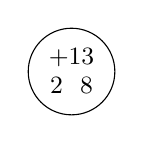
\begin{tikzpicture}[baseline=-0.5ex]
\draw (0,0) circle (0.55);
\node at (0,0.18) {\small $+13$};
\node at (0,-0.18) {\small $2\ \ 8$};
\end{tikzpicture}；相同电子数（10 e\textsuperscript{$-$}) 的四核微粒：\ch{NH3} 或 \ch{CH4}（答案给的是 \ch{PH3}，疑为 \ch{NH3} 之误）；
\item \textcircled{1} $x = 92.18$\%，$y = 4.72$\%（原卷参考答案写作“83.18；13.72”，按算式复核应为上述数值）；\textcircled{2} $>$；0.19 g。
\end{enumerate}

\item
\begin{enumerate}[label=（\arabic*）]
\item CD；
\item $1\times 10^{-9} \sim 1\times 10^{-7}$ m；丁达尔效应；
\item 阳；胶体粒子带负电荷，通电发生电泳向阳极移动；
\item 胶体遇其他电解质溶液发生了聚沉；
\item AD；
\item B；
\item 不稳定，易受外界环境影响。
\end{enumerate}

\item
\begin{enumerate}[label=（\arabic*）]
\item 28 g$\cdot$mol\textsuperscript{$-$1}；$0.5N_A$；
\item A；
\item D；
\item A（原卷参考答案写作“B”，按物理推算应为 A：等质量下 $V\propto 1/\rho$，$\rho(\mathrm{CO_2})=1.96$ 最大，故 \ch{CO2} 气球最小）；
\item 6.72 L；2.8 g；
\item \textcircled{1} 0.5 mol；\textcircled{2} 34.4 g/mol；\textcircled{3} 8.8 g；
\item B；
\item C；
\item AC。
\end{enumerate}

\item
\begin{enumerate}[label=（\arabic*）]
\item 0.154；
\item 1.70；
\item C；100 mL 容量瓶；
\item 搅拌，加速溶解；引流，防止溶液漏出；
\item C；
\item 0.146；
\item A。
\end{enumerate}

\item
\begin{enumerate}[label=（\arabic*）]
\item B；
\item C；
\item B；
\item CD；
\item $\mathrm{NaHCO_3 + NaHSO_4 \longrightarrow Na_2SO_4 + H_2O + CO_2 \uparrow}$；
\item 9.85；
\item 硫酸氢钠和硫酸钠；
\item 蓝。
\end{enumerate}
\end{enumerate}
\fi

\end{document}
"

\documentclass[11pt,a4paper]{article}
\usepackage{chem}

% ---- 卷名（页眉；答案版自动追加版本标记）----
\newcommand{\paperhead}{2025-2026 学年上海交大附中高一（上）月考化学试卷（10 月份）}
\fancyhead[L]{\small\kaishu \paperhead\vermark}

% ---- 标题 ----
\title{\heiti\bfseries\Large \paperhead}
\author{}
\date{}

\begin{document}
\maketitle
\thispagestyle{fancy}

%==========================================================
\bigsection{一、破解月壤化学之谜（20 分）}

\noindent\textbf{1.（20 分）}2025 年 7 月，中国科学家基于对月壤样品的成分分析，于《自然》期刊上发表了突破性研究，其中所揭示的数据为理解月球背面的岩浆活动、水含量及撞击历史提供了关键证据。

\begin{enumerate}[label=（\arabic*）]
\item \ch{^{3}He} 与 \ch{^{3}H} 发生聚变有可能被开发为能源。\ch{^{3}He} 与 \ch{^{3}H} 具有相同的\blank[2.4em]。
\choice{中子数}{质子数}{质量数}{电子数}

\item 月壤中含有的元素可形成 \ch{^{13}C^{17}O} 分子，有助于揭示行星诞生之谜，下列关于 \ch{^{13}C^{17}O} 和 \ch{^{12}C^{16}O} 的说法正确的是\blank[2.4em]。
\choice{互为同素异形体}{互为同位素}{具有相同的性质}{它们是同种物质}

\item 月壤的构成与地球土壤类似。土壤中含有的 W、X、Y、Z 是 1$\sim$18 号元素中的四种，且原子序数依次增大，最外层电子数之和为 15，其中 W 的最外层电子数是内层电子总数的 3 倍，X、Y、Z 原子序数是连续的。

写出 W 元素的简单离子的电子式\blank[6em]。

\item X 原子核外电子所占据的电子层中，能量最高的是\blank[2.5em]层（填符号）。

\item Y 元素的简单离子结构示意图为\blank[3em]。请写出与它具有相同电子数的四核微粒的化学式\blank[2.5em]（写一个即可）。

\item Z 元素在自然界中有三种稳定的同位素，相关信息如下：

\begin{center}
\begin{tabular}{|c|c|c|c|}
\hline
\rule{0pt}{1.2em}核素符号 & \ch{^{28}Z} & \ch{^{29}Z} & \ch{^{30}Z} \\
\hline
\rule{0pt}{1.2em}相对原子质量 & 27.977 & 28.976 & 29.974 \\
\hline
\rule{0pt}{1.2em}丰度（\%） & $x$ & $y$ & 3.10 \\
\hline
\rule{0pt}{1.2em}Z 元素的平均相对原子质量 & \multicolumn{3}{c|}{28.086} \\
\hline
\end{tabular}
\end{center}

\textcircled{1} 表格中 $x$、$y$ 和 3.10\% 分别代表 Z 中对应核素的丰度，则 $x =$\blank[3.5em] \%，$y =$\blank[3.5em] \%（计算结果保留两位小数）。

\textcircled{2} \ch{^{30}Z} 在自然界的质量分数\blank[2em]3.1\%（填“>”、“<”或“=”），12 g ZO\textsubscript{2} 中 \ch{^{30}Z} 的质量为\blank[3em]（计算结果保留两位小数）。
\end{enumerate}

%==========================================================
\bigsection{二、胶体金检测试剂（20 分）}

\noindent\textbf{2.（20 分）}胶体金（Au）免疫层析法可用于快速检测新型冠状病毒抗体。利用柠檬酸钠溶液还原氯金酸（\ch{HAuCl4}）即可制备得到胶体金。研究发现：柠檬酸钠的用量不同会导致胶体金粒径和颜色的不同。免疫胶体金技术可用于甲型流感病毒的快速免疫筛查，检测原理是胶体金与蛋白质分子的正电荷基团形成牢固的结合体，再通过抗原-抗体结合形成免疫复合物，使得胶体金颗粒聚集，发生颜色变化。

\begin{enumerate}[label=（\arabic*）]
\item 下列说法中错误的是\blank[3em]。
\choice{胶体金颗粒带负电荷}{用半透膜分离胶体金吸附的离子}{胶体金颗粒的团聚过程利用电泳原理}{检测过程胶体金分散质粒子直径不变}

\item 利用超显微镜，可以观察到胶体金颗粒的形态，胶体金分散质粒子的直径大致范围在\blank[4em]m 之间。检验胶体最便利的方法是观察它\blank[4em]。

\item 若将胶体金装入 U 型管中，插入电极后通直流电，发现\blank[2.5em]极（选填“阴”或“阳”）附近颜色加深，产生这一现象的原因是\blank[8em]。

\item 向新冠肺炎自测试剂盒中倒入可乐或柠檬水可能会导致假阳性。推测这一现象的原因：\par\noindent\hspace{2em}\blank[10em]。

\item 与第（4）题现象的原理相同的选项有\blank[3em]。
\choice{长江三角洲的形成}{血液透析}{大雨过后拍到“耶稣光”}{不同品牌的墨水不能混用}

\item 已知等浓度的 \ch{MgSO4} 溶液对胶体金的聚沉效果强于 \ch{NaCl} 溶液，加入等浓度的下列溶液时，聚沉胶体金效果最明显的是\blank[3em]。
\choice{\ch{BaCl2}}{\ch{Al2(SO4)3}}{\ch{KCl}}{\ch{CuSO4}}

\item 请分析该公司根据胶体金免疫层析法研制自测试剂盒的缺陷：\blank[10em]。
\end{enumerate}

%==========================================================
\bigsection{三、物质的量（22 分）}

\noindent\textbf{3.（22 分）}研究含碳物质的转化，对缓解能源危机和实现碳中和具有重要意义。碳和甲烷均可以与水反应用来制取水煤气（\ch{CO}、\ch{H2}），请回答下列问题：

\begin{enumerate}[label=（\arabic*）]
\item 标准状况下，11.2 L \ch{CO} 的摩尔质量为\blank[3.5em]g$\cdot$mol\textsuperscript{$-1$}，分子个数为\blank[4em]。

\item 1 mol \ch{CH4} 中含有的 H 原子个数与\blank[3em]g \ch{H2O} 中含有的 H 原子个数相同。
\choice{36}{18}{72}{9}

\item 下列叙述错误的是\blank[3em]。
\begin{itemize}[leftmargin=2em,itemsep=0.1em]
\item[ \textcircled{1} ] 摩尔是国际单位制中的七个基本物理量之一；
\item[ \textcircled{2} ] 1 mol 任何物质都含有约 $6.02\times 10^{23}$ 个原子；
\item[ \textcircled{3} ] $6.02\times 10^{23}$ 就是阿伏加德罗常数；
\item[ \textcircled{4} ] 碳原子的摩尔质量是 12 g；
\item[ \textcircled{5} ] \ch{CO2} 的摩尔质量等于 1 mol \ch{CO2} 分子的质量；
\item[ \textcircled{6} ] 1 mol \ch{CO2} 中含有 1 mol 碳和 2 mol 氧；
\item[ \textcircled{7} ] 0.012 kg \ch{^{12}C} 中含有 \ch{^{12}C} 的数目为 1 mol。
\end{itemize}
\choice{\textcircled{1}\textcircled{2}\textcircled{3}}{\textcircled{2}\textcircled{3}\textcircled{4}}{\textcircled{2}\textcircled{3}\textcircled{4}\textcircled{6}}{全部}

\item 常温常压下，用等质量的 \ch{CH4}、\ch{CO}、\ch{H2}、\ch{CO2} 四种气体分别吹出四个气球。其中气体为 \ch{CO2} 的是\blank[3em]（填序号）。

\begin{center}
\begin{tikzpicture}
  % 原卷图（截图裁切自 img_2，二值化放大 2 倍）
  \node[anchor=south west,inner sep=0] (img) at (0,0)
    {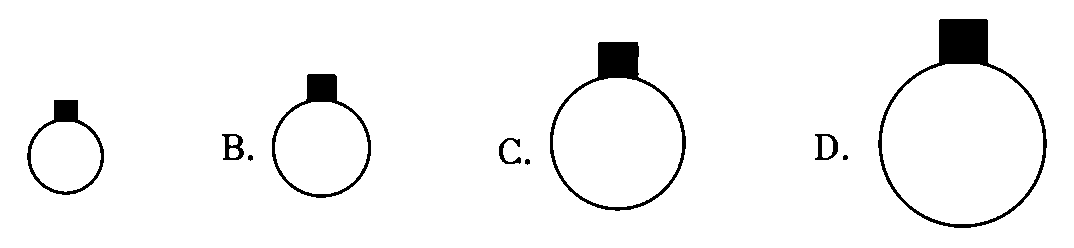
\includegraphics[width=0.80\textwidth]{figures/balloons.png}};
  % 原卷图中未印字母，此处按气球中心位置补注 A/B/C/D
  \foreach \lab/\p in {A/0.0615, B/0.2980, C/0.5754, D/0.8957} {
    \node[below=2pt] at ($(img.south west)!\p!(img.south east)$) {\small\textbf{\lab}};
  }
\end{tikzpicture}
\end{center}

\item 标准状况下，8.96 L \ch{CH4} 和 \ch{CO} 的混合气体总质量为 7.6 g，则混合气体中甲烷的体积为\blank[3em]L，一氧化碳的质量为\blank[3em]g。

\item 同温同压下，17.2 g \ch{N2}、\ch{CO} 和 \ch{CO2} 的混合气体与 4.4 g \ch{CO2} 的体积之比为 5:1。
\begin{enumerate}[label=\textcircled{\arabic*}]
\item 该混合气体的总物质的量为\blank[3em]mol。
\item 该混合气体的平均摩尔质量为\blank[3em]g/mol。
\item 该混合气体中 \ch{CO2} 的质量为\blank[3em]g。
\end{enumerate}

制取水煤气的副产品为 \ch{CO2}，工业中可以利用 \ch{CO2} 合成纯碱。

现有一份纯碱样品，已知其中只含有氯化钠杂质。某化学实验小组为测定样品中碳酸钠的含量进行如下实验：

\noindent 步骤 I：准确称量 21.20 g 纯碱样品，加入适量蒸馏水溶解；\\
步骤 II：向上述溶液中逐滴加入 \ch{CaCl2} 溶液，直至不再产生沉淀为止；\\
步骤 III：将所得混合物过滤、洗涤、干燥，得到 15.00 g 固体。

请计算：

\item 步骤 III 中所得固体的物质的量为\blank[3em]mol。
\choice{0.3}{0.15}{15}{0.135}

\item 样品中 \ch{Na2CO3} 的质量分数为\blank[3em]。
\choice{70.8\%}{78.5\%}{75\%}{25\%}

\item 下列实验方案中，能测定样品中碳酸钠质量分数的是\blank[3em]（双选）。
\begin{itemize}[leftmargin=2em,itemsep=0.1em]
\item[A.] 向步骤 I 所得溶液逐滴加入标准盐酸至恰好不再有气体生成，共消耗 $b$ mol 溶质的稀盐酸。经计算，测得样品中 \ch{Na2CO3} 的质量分数为 $\omega(\ch{Na2CO3}) = \dfrac{53b}{21.20}$。
\item[B.] 向步骤 I 所得溶液中加入足量稀硫酸，将生成的气体用碱石灰吸收，碱石灰增重 $a$ g。经计算，测得样品中 \ch{Na2CO3} 的质量分数为 $\omega(\ch{Na2CO3}) = \dfrac{53a}{22\times 21.20}$。
\item[C.] 向步骤 I 所得溶液中加入硝酸酸化，再加入足量的硝酸银溶液充分反应，过滤、洗涤、干燥，得 $c$ g 固体。经计算，测得样品中 \ch{Na2CO3} 的质量分数为 $\omega(\ch{Na2CO3}) = \left(1 - \dfrac{58.5c}{143.5\times 21.20}\right)$。
\end{itemize}
\end{enumerate}

%==========================================================
\bigsection{四、生理盐水中氯化钠含量的分析（19 分）}

\noindent\textbf{4.（19 分）}生理盐水是渗透压与动物或人体血浆相等的氯化钠溶液，其质量分数为 0.9\%，广泛用于补液，体外细胞培养及医疗操作中。

\begin{enumerate}[label=（\arabic*）]
\item 请计算生理盐水的物质的量浓度为\blank[3.5em]mol/L。（生理盐水密度约等于 1 g/cm\textsuperscript{3}，结果保留三位有效数字）

某同学想要使用如下方法对某市售生理盐水进行浓度分析：
\begin{itemize}[leftmargin=2em,itemsep=0.1em]
\item[ \textcircled{1} ] 配制 0.1000 mol/L 硝酸银溶液 100 mL
\item[ \textcircled{2} ] 取 25.00 mL 生理盐水于锥形瓶中，加入指示剂后使用配制好的硝酸银溶液进行滴定，消耗 36.62 mL。
\end{itemize}
滴定过程中发生的反应：$\mathrm{Ag^{+} + Cl^{-} \longrightarrow AgCl \downarrow}$

\item 计算需称取硝酸银\blank[3.5em]g（结果保留三位有效数字）。

\item 在配制硝酸银溶液实验中，下列不需要使用的仪器是\blank[3em]（填选项），除了玻璃棒和下列选项中出现的仪器外，还需要的玻璃仪器是\blank[4em]。
\choice{250 mL 烧杯}{胶头滴管}{量筒}{电子天平}

\item 配制过程中，玻璃棒使用了两次，其作用分别为\blank[6em]、\blank[6em]。

\item 下列配制硝酸银溶液的主要操作步骤，正确顺序是\blank[3em]。
\begin{itemize}[leftmargin=2em,itemsep=0.1em]
\item[ \textcircled{1} ] 称取一定质量的硝酸银，放入烧杯中，用适量蒸馏水溶解；
\item[ \textcircled{2} ] 加水至液面刻度线下 1$\sim$2 厘米时，改用胶头滴管加蒸馏水至凹液面与刻度线相切；
\item[ \textcircled{3} ] 将溶液转移到容量瓶中；
\item[ \textcircled{4} ] 盖好瓶塞，反复上下颠倒，摇匀；
\item[ \textcircled{5} ] 用少量蒸馏水洗涤烧杯内壁和玻璃棒 2$\sim$3 次，洗涤液转移到容量瓶中。
\end{itemize}
\choice{\textcircled{1}\textcircled{5}\textcircled{3}\textcircled{2}\textcircled{4}}{\textcircled{1}\textcircled{3}\textcircled{2}\textcircled{4}\textcircled{5}}{\textcircled{1}\textcircled{5}\textcircled{3}\textcircled{2}\textcircled{4}}{\textcircled{1}\textcircled{3}\textcircled{5}\textcircled{4}\textcircled{2}}

\item 计算该市售生理盐水的物质的量浓度为\blank[3.5em]mol/L（密度约等于 1 g$\cdot$cm\textsuperscript{$-$3}，结果保留三位有效数字）。

\item 溶液中微粒的总浓度越大，溶液的渗透压越高。人体的血细胞在高渗透压的溶液中会失水皱缩，在低渗透压环境下会吸水膨胀，只有在等渗透压溶液中才能够保持正常。因此诸如生理盐水这样的等渗溶液十分重要。已知 \ch{NaCl} 在溶液中的存在形式为 \ch{Na+} 与 \ch{Cl-}，\ch{Na2SO4} 在溶液中的存在形式为 \ch{Na+} 与 $\mathrm{SO_4^{2-}}$，试判断在 0.12 mol/L 的 \ch{Na2SO4} 溶液中血细胞会怎样：\blank[3em]。
\choicethree{失水皱缩}{吸水膨胀}{保持正常}
\end{enumerate}

%==========================================================
\bigsection{五、紫甘蓝指示剂（18 分）}

\noindent\textbf{5.（19 分）}紫甘蓝与石蕊类似，在酸碱性不同的溶液中均能显示出不同的颜色，因此也被作为酸碱指示剂。以下是紫甘蓝指示剂随溶液 pH 值的变色范围。

\begin{center}
\begin{tabular}{|c|c|c|c|c|c|c|c|}
\hline
\rule{0pt}{1.2em}pH & 1 & 2$\sim$3 & 4$\sim$6 & 7$\sim$9 & 10 & 11 & 12$\sim$14 \\
\hline
\rule{0pt}{1.2em}溶液颜色 & 深红 & 紫红 & 浅紫 & 蓝 & 青 & 绿 & 黄 \\
\hline
\end{tabular}
\end{center}

\begin{enumerate}[label=（\arabic*）]
\item 下列可能使紫甘蓝溶液变为浅紫色的物质有\blank[3em]。
\choice{\ch{NaCl}}{\ch{CH3COOH}}{\ch{Ca(OH)2}}{\ch{K2SO4}}

向一定浓度的碳酸氢钠中滴加几滴紫甘蓝溶液，观察到溶液呈蓝色。向溶液中滴加几滴稀盐酸，观察到有气泡产生，且溶液依然呈蓝色。

\item 碳酸氢钠属于\blank[3em]。
\choice{正盐}{碱式盐}{酸式盐}{复盐}

\item 滴加稀盐酸前的碳酸氢钠溶液呈\blank[3em]。
\choicethree{酸性}{碱性}{中性}

向一定浓度的硫酸氢钠中滴加几滴紫甘蓝溶液，观察到溶液呈紫红色。向溶液中滴加几滴稀硫酸，无明显现象。另取少量硫酸氢钠溶液滴加到碳酸氢钠溶液中，观察到有气泡产生。

\item 下列说法正确的是\blank[3em]。
\choice{硫酸氢钠不是酸式盐}{硫酸氢钠溶液呈碱性}{某些盐类物质可以互相反应}{酸式盐可能显酸性可能显碱性}

\item 写出硫酸氢钠与碳酸氢钠溶液反应的化学方程式\blank[10em]。

向盛有 0.2 mol 硫酸氢钠溶液的烧杯中加入碳酸钡固体，当加入 $a$ g 碳酸钡固体后，产生了 0.05 mol 气体（假设 \ch{CO2} 全部逸出）。

\item $a =$\blank[4em]。

\item 此时溶液中的溶质为\blank[6em]。

\item 继续加入碳酸钡固体，当烧杯中恰好有 23.3 g 固体时，向烧杯中滴加几滴紫甘蓝溶液，溶液呈\blank[2em]色。
\end{enumerate}

%==========================================================
% 以下「参考答案」整节仅在答案版输出（试卷版由 \ifanswer 整段吞掉）
\ifanswer
\newpage
\bigsection{参考答案}

\begin{enumerate}[label=\textbf{\arabic*.},leftmargin=2.5em]
\item
\begin{enumerate}[label=（\arabic*）]
\item A（原卷参考答案写作“A”；\ch{^{3}He} 与 \ch{^{3}H} 的中子数为 1 与 2、质子数为 2 与 1，均不相同，相同的是质量数 3，按题意应为 C）；
\item D；
\item $\left[:\ddot{\mathrm{O}}:\right]^{2-}$（O\textsuperscript{2-} 的电子式）；
\item M；
\item Al\textsuperscript{3+} 的结构示意图为
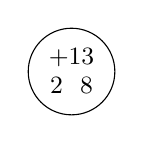
\begin{tikzpicture}[baseline=-0.5ex]
\draw (0,0) circle (0.55);
\node at (0,0.18) {\small $+13$};
\node at (0,-0.18) {\small $2\ \ 8$};
\end{tikzpicture}；相同电子数（10 e\textsuperscript{$-$}) 的四核微粒：\ch{NH3} 或 \ch{CH4}（答案给的是 \ch{PH3}，疑为 \ch{NH3} 之误）；
\item \textcircled{1} $x = 92.18$\%，$y = 4.72$\%（原卷参考答案写作“83.18；13.72”，按算式复核应为上述数值）；\textcircled{2} $>$；0.19 g。
\end{enumerate}

\item
\begin{enumerate}[label=（\arabic*）]
\item CD；
\item $1\times 10^{-9} \sim 1\times 10^{-7}$ m；丁达尔效应；
\item 阳；胶体粒子带负电荷，通电发生电泳向阳极移动；
\item 胶体遇其他电解质溶液发生了聚沉；
\item AD；
\item B；
\item 不稳定，易受外界环境影响。
\end{enumerate}

\item
\begin{enumerate}[label=（\arabic*）]
\item 28 g$\cdot$mol\textsuperscript{$-$1}；$0.5N_A$；
\item A；
\item D；
\item A（原卷参考答案写作“B”，按物理推算应为 A：等质量下 $V\propto 1/\rho$，$\rho(\mathrm{CO_2})=1.96$ 最大，故 \ch{CO2} 气球最小）；
\item 6.72 L；2.8 g；
\item \textcircled{1} 0.5 mol；\textcircled{2} 34.4 g/mol；\textcircled{3} 8.8 g；
\item B；
\item C；
\item AC。
\end{enumerate}

\item
\begin{enumerate}[label=（\arabic*）]
\item 0.154；
\item 1.70；
\item C；100 mL 容量瓶；
\item 搅拌，加速溶解；引流，防止溶液漏出；
\item C；
\item 0.146；
\item A。
\end{enumerate}

\item
\begin{enumerate}[label=（\arabic*）]
\item B；
\item C；
\item B；
\item CD；
\item $\mathrm{NaHCO_3 + NaHSO_4 \longrightarrow Na_2SO_4 + H_2O + CO_2 \uparrow}$；
\item 9.85；
\item 硫酸氢钠和硫酸钠；
\item 蓝。
\end{enumerate}
\end{enumerate}
\fi

\end{document}
